% Created 2024-04-22 lun 18:22
% Intended LaTeX compiler: pdflatex
\documentclass[aspectratio=169, usenames,svgnames,dvipsnames]{beamer}
\usepackage[utf8]{inputenc}
\usepackage[T1]{fontenc}
\usepackage{graphicx}
\usepackage{longtable}
\usepackage{wrapfig}
\usepackage{rotating}
\usepackage[normalem]{ulem}
\usepackage{amsmath}
\usepackage{amssymb}
\usepackage{capt-of}
\usepackage{hyperref}
\usepackage{color}
\usepackage{listings}
\usepackage{mathpazo}
\usepackage{gensymb}
\usepackage{amsmath}
\usepackage{diffcoeff}
\usepackage{steinmetz}
\usepackage{mathtools}
\usepackage{fancyvrb}
\DefineVerbatimEnvironment{verbatim}{Verbatim}{fontsize=\tiny, formatcom = {\color{black!70}}}
\bibliographystyle{plain}
\usepackage{siunitx}
\sisetup{per-mode=symbol}
\sisetup{output-decimal-marker={,}}
\DeclareSIUnit{\watthour}{Wh}
\DeclareSIUnit{\wattpeak}{Wp}
\DeclareSIUnit{\watthour}{Wh}
\DeclareSIUnit{\amperehour}{Ah}
\usepackage{steinmetz}
\hypersetup{colorlinks=true, linkcolor=Blue, urlcolor=Blue}
\usepackage[symbol, perpage]{footmisc}
\parskip=5pt
\usetheme{Boadilla}
\usecolortheme{rose}
\usefonttheme{serif}
\author{\href{https://oscarperpinan.github.io}{Oscar Perpiñán Lamigueiro}}
\date{}
\title{Análisis de datos de producción}
\subtitle{Energía Solar Fotovoltaica}
\institute[UPM]{Universidad Politécnica de Madrid}
\setbeamercolor{alerted text}{fg=blue!50!black} \setbeamerfont{alerted text}{series=\bfseries}
\AtBeginSubsection[]{\begin{frame}[plain]\tableofcontents[currentsubsection,sectionstyle=show/hide,subsectionstyle=show/shaded/hide]\end{frame}}
\AtBeginSection[]{\begin{frame}[plain]\tableofcontents[currentsection,hideallsubsections]\end{frame}}
\beamertemplatenavigationsymbolsempty
\setbeamertemplate{footline}[frame number]
\setbeamertemplate{itemize items}[triangle]
\setbeamertemplate{enumerate items}[circle]
\setbeamertemplate{section in toc}[circle]
\setbeamertemplate{subsection in toc}[circle]
\hypersetup{
 pdfauthor={\href{https://oscarperpinan.github.io}{Oscar Perpiñán Lamigueiro}},
 pdftitle={Análisis de datos de producción},
 pdfkeywords={},
 pdfsubject={},
 pdfcreator={Emacs 29.2 (Org mode 9.6.23)}, 
 pdflang={Spanish}}
\begin{document}

\maketitle

\begin{frame}[label={sec:org67ee9b7}]{Planteamiento}
\begin{itemize}
\item La \alert{energía producida por un SFV} durante un período puede ser \alert{estimada} a partir de la \alert{radiación incidente} y de las \alert{características técnicas} del sistema.
\item Teniendo en cuenta el carácter estocástico de la radiación solar, la estimación de la energía que producirá un SFV durante los próximos años es un ejercicio de \alert{predicción con incertidumbre} asociada.
\item El funcionamiento de un SFV puede ser analizado tomando esta estimación como referencia (\alert{comparación modelo-medidas}).
\item En el caso de centrales FV, se pueden detectar problemas de funcionamiento comparando diferentes partes de la central (\alert{coherencia estadística}).
\end{itemize}
\end{frame}

\section{Estadística}
\label{sec:org27eca0c}


\begin{frame}[label={sec:org8a74808}]{Variable aleatoria y proceso estocástico}
\begin{itemize}
\item Una \alert{variable aleatoria} es una función que asigna un único numero
real a cada resultado de un espacio muestral en un experimento.
\item Un \alert{proceso estocástico} es una variable aleatoria que evoluciona a
lo largo del \alert{tiempo} (p.ej. la radiación).
\end{itemize}
\end{frame}


\begin{frame}[label={sec:org24b3f53}]{Función de densidad de probabilidad}
La función de densidad de probabilidad, \(f(X)\), de una variable
aleatoria \alert{asigna probabilidad} a un suceso:

\begin{columns}
\begin{column}{0.5\columnwidth}

\[
P(a<X<b)=\int_{a}^{b}f(x)dx
\]


\[
P(X<b)=\int_{-\infty}^{b}f(x)dx\]


\[
P(X>a)=\int_{a}^{\infty}f(x)dx\]
\end{column}

\begin{column}{0.5\columnwidth}
\begin{center}
\includegraphics[height=0.7\textheight]{../figs/FuncionDensidadProbabilidad.pdf}
\end{center}
\end{column}
\end{columns}
\end{frame}


\begin{frame}[label={sec:org3ca4441}]{Media, varianza y desviación estándar}
\begin{itemize}
\item La \alert{media} de una variable aleatoria es el \alert{centro de masas} de su función densidad de probabilidad:
\end{itemize}

\[
\mu_{X}=\int_{-\infty}^{\infty}x\cdot f(x)dx
\]

\begin{itemize}
\item La \alert{varianza} de una variable aleatoria es la \alert{media del cuadrado de las desviaciones} respecto a la media:
\end{itemize}

\[
\sigma_{X}^{2}=\int_{-\infty}^{\infty}(x-\mu_{X})^{2}\cdot f(x)dx
\]

\begin{itemize}
\item La \alert{desviación estándar} es la raiz cuadrada de la varianza: \(\sigma_{X}=\sqrt{\sigma_{X}^2}\)
\end{itemize}
\end{frame}



\begin{frame}[label={sec:org675d2d7}]{Combinación lineal de variables aleatorias}
\begin{itemize}
\item La \alert{media de la suma} de varias variables aleatorias \alert{independientes} es
la suma de las medias:
\end{itemize}
\[
\mu_{X_{1}+...+X_{n}}=\mu_{X_{1}}+...+\mu_{X_{n}}
\]

\begin{itemize}
\item La \alert{varianza de la \emph{suma o resta}} de varias variables aleatorias
\alert{independientes} es la \alert{suma} de las varianzas:
\end{itemize}

\[
\sigma_{X_{1}\pm...\pm X_{n}}^{2}=\sigma_{X_{1}}^{2}+...+\sigma_{X_{n}}^{2}
\]
\end{frame}



\begin{frame}[label={sec:orge604e07}]{Media y varianza de la media muestral}
\begin{itemize}
\item Una \alert{muestra de una población} es un conjunto de variables
aleatorias independientes (\(X_{1}...X_{n}\)).

\item Si se toma una muestra de una población, la media de la muestra es otra
variable aleatoria (que es una suma de variables aleatorias)
\end{itemize}

\[
\overline{X}=\frac{1}{n}\sum_{i=n}X_{i}
\]
\end{frame}



\begin{frame}[label={sec:orgb79179c}]{Media y varianza de la media muestral}
Sea una población cuya media es \(\mu\) y su varianza es \(\sigma^{2}\):

\begin{itemize}
\item La \alert{media de la media muestral} es la media poblacional:
\end{itemize}
\[
\mu_{\overline{X}}=\frac{1}{n}\sum_{i = n}\mu_{X_{i}} = \mu
\]

\begin{itemize}
\item La \alert{varianza de la media muestral} es la varianza poblacional dividido por el número de muestras.
\end{itemize}

\[
\sigma_{\overline{X}}^{2}=\sigma_{\frac{1}{n}X_{1}}^{2}+...+\sigma_{\frac{1}{n}X_{n}}^{2}=\frac{\sigma^2}{N}
\]

\begin{block}{}
Por tanto, una forma de \alert{reducir la incertidumbre} es realizar la
\alert{medida en repetidas ocasiones}.
\end{block}
\end{frame}



\begin{frame}[label={sec:orgd25f928}]{Mediana y cuartiles}
\begin{columns}
\begin{column}{0.5\columnwidth}
\begin{itemize}
\item La \alert{mediana} divide el conjunto de valores de la variable en \alert{dos
mitades} iguales (divide el area encerrada por la función densidad
de probabilidad en dos partes iguales).
\item Los \alert{cuartiles} dividen este area en \alert{cuatro} partes iguales.
\item El area encerrada entre cada par de cuartiles es igual al 25\% del total.
\item La \alert{mediana} es el \alert{segundo cuartil}.
\item La \alert{distancia intercuartil} (definida entre los cuartiles 1 y 3) es
una \alert{medida de la dispersión} de la variable.
\end{itemize}
\end{column}

\begin{column}{0.5\columnwidth}
\begin{center}
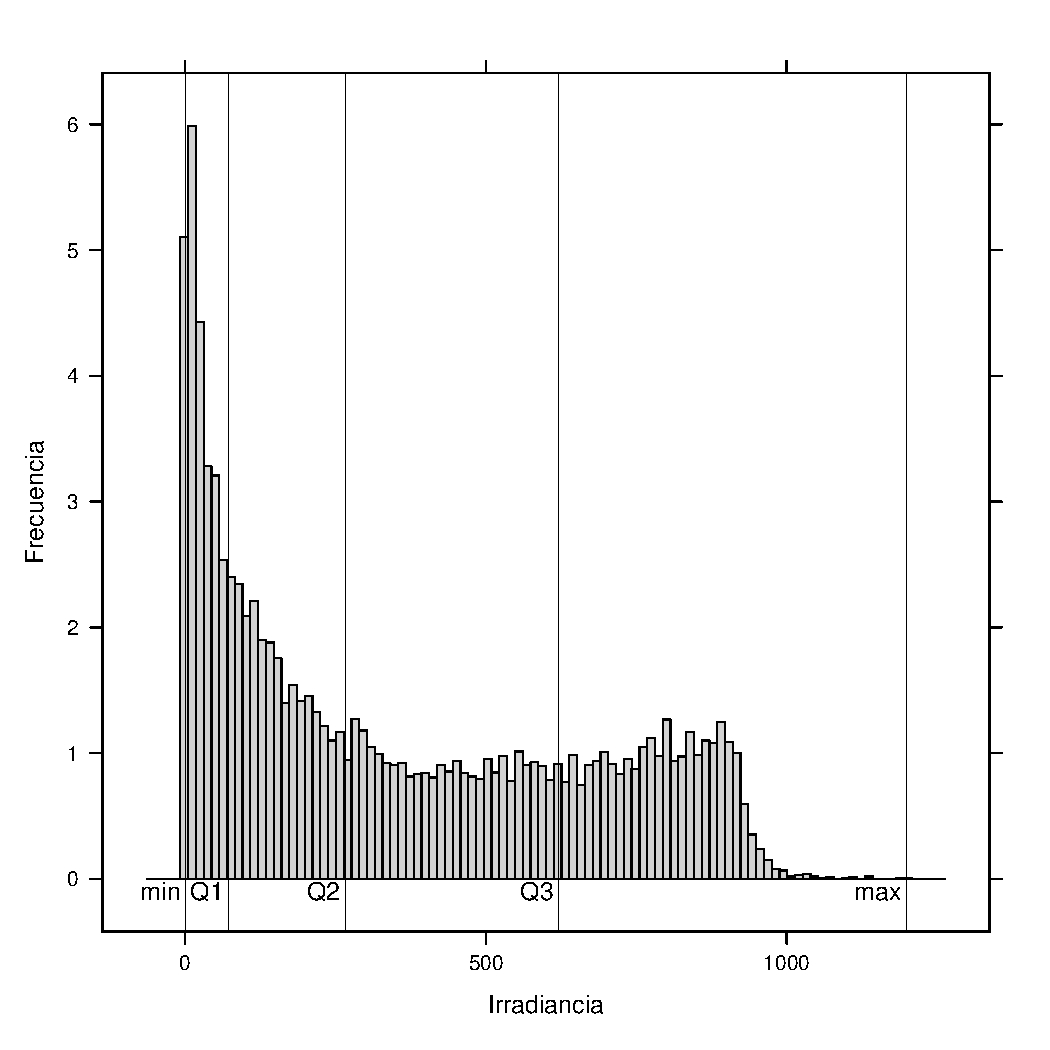
\includegraphics[height=0.9\textheight]{../figs/cuantiles.pdf}
\end{center}
\end{column}
\end{columns}
\end{frame}

\section{Gráficos estadísticos}
\label{sec:org90610a4}


\begin{frame}[label={sec:orgdd805aa}]{Función de Densidad de Probabilidad}
\begin{center}
\includegraphics[height=0.9\textheight]{../figs/FuncionDensidadProbabilidad.pdf}
\end{center}
\end{frame}

\begin{frame}[label={sec:org843828f}]{Histograma}
\begin{center}
\includegraphics[height=0.9\textheight]{../figs/Histograma.pdf}
\end{center}
\end{frame}


\begin{frame}[label={sec:org14eb7e4}]{Gráficos boxplot}
\begin{columns}
\begin{column}{0.5\columnwidth}
\begin{itemize}
\item Línea central: mediana (Q2).
\item Límites de la caja: cuantiles Q1 y Q2 (IQR)
\item Bigotes: valores máximo y mínimo o 1.5·IQR.
\item Puntos: valores anómalos (\emph{outliers}).
\end{itemize}
\end{column}

\begin{column}{0.5\columnwidth}
\begin{center}
\includegraphics[height=0.9\textheight]{../figs/GraficoBoxplot.pdf}
\end{center}
\end{column}
\end{columns}
\end{frame}

\begin{frame}[label={sec:orgbf3bd7f}]{Gráficos de dispersión}
\begin{center}
\includegraphics[height=0.9\textheight]{../figs/GraficoDispersion.pdf}
\end{center}
\end{frame}


\begin{frame}[label={sec:orgd3ccf0b}]{Matrices de gráficos de dispersión}
\begin{center}
\includegraphics[height=0.9\textheight]{../figs/Splom.png}
\end{center}
\end{frame}

\section{Gráficos Fotovoltaicos}
\label{sec:orge00dd86}

\begin{frame}[label={sec:orga8c00e3}]{Inventario\footnote{Más ejemplos en el informe \guillemotleft{}\href{https://iea-pvps.org/key-topics/analytical-monitoring-of-pv-systems-final/}{Analytical Monitoring of Grid-connected Photovoltaic Systems}\guillemotright{} de la Task 13 del IEA-PVPS.}}
\begin{itemize}
\item \(Y_f \sim Y_r\) 

Detección de sombreado, defectos en cableado DC y AC, fallos o limitación del inversor.

\item \(Y_a \sim Y_r\)

Detección de sombreado o defectos en cableado DC.

\item \(pr \sim T_c\) 

Detección de sombreado, degradación, o puntos calientes.

\item \((T_c - T_a) \sim y_r\)

Detección de problemas de disipación de calor.

\item \(V_G \sim T_c\)

Detección de problemas en el MPPT, limitación del inversor, diodos de bypass.
\end{itemize}
\end{frame}

\begin{frame}[label={sec:org90d143c}]{\(Y_f \sim Y_r\)}
\begin{columns}
\begin{column}{0.3\columnwidth}
\begin{itemize}
\item Valores diarios e intradiarios.
\item Relación lineal creciente.
\item Detección de sombreado, defectos en cableado DC y AC, fallos o limitación del inversor.
\end{itemize}
\end{column}

\begin{column}{0.7\columnwidth}
\begin{center}
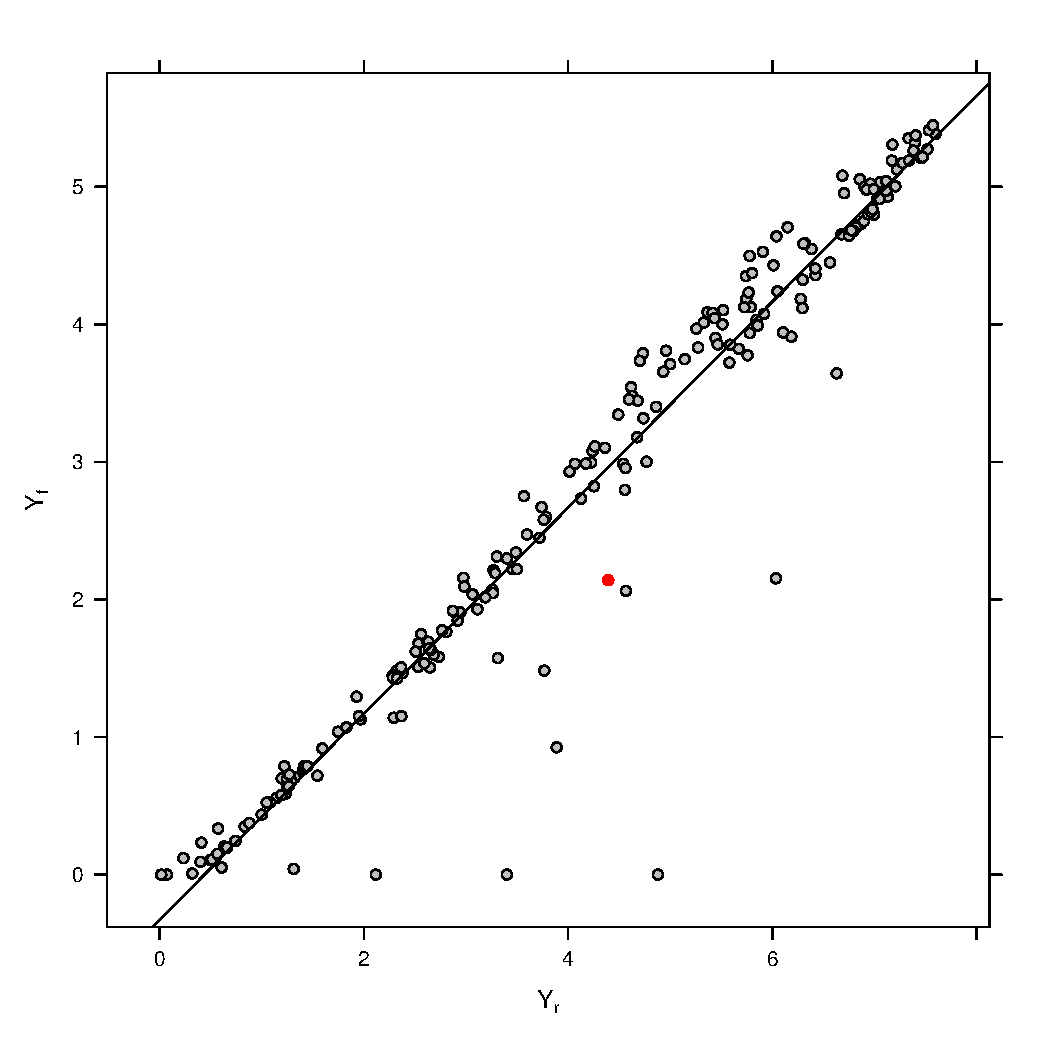
\includegraphics[height=0.95\textheight]{../figs/YfYr.pdf}
\end{center}
\end{column}
\end{columns}
\end{frame}

\begin{frame}[label={sec:org90baebc}]{Error de funcionamiento \(Y_f \sim Y_r\)}
\begin{center}
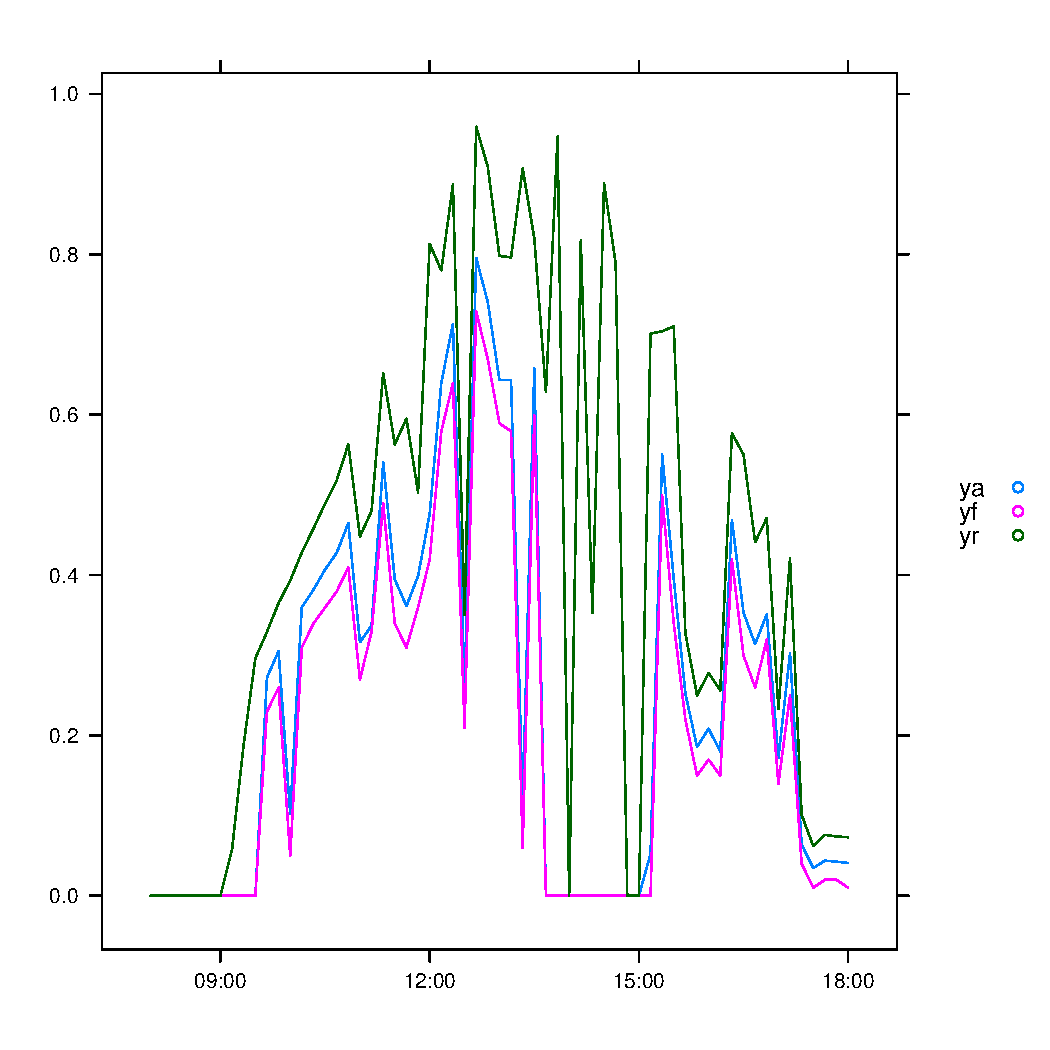
\includegraphics[height=0.95\textheight]{../figs/ErrorYf.pdf}
\end{center}
\end{frame}

\begin{frame}[label={sec:orgaf9ecb1}]{\(Y_a \sim Y_r\)}
\begin{columns}
\begin{column}{0.3\columnwidth}
\begin{itemize}
\item Valores diarios e intradiarios.
\item Relación lineal creciente.
\item Detección de sombreado o defectos en cableado DC.
\end{itemize}
\end{column}

\begin{column}{0.7\columnwidth}
\begin{center}
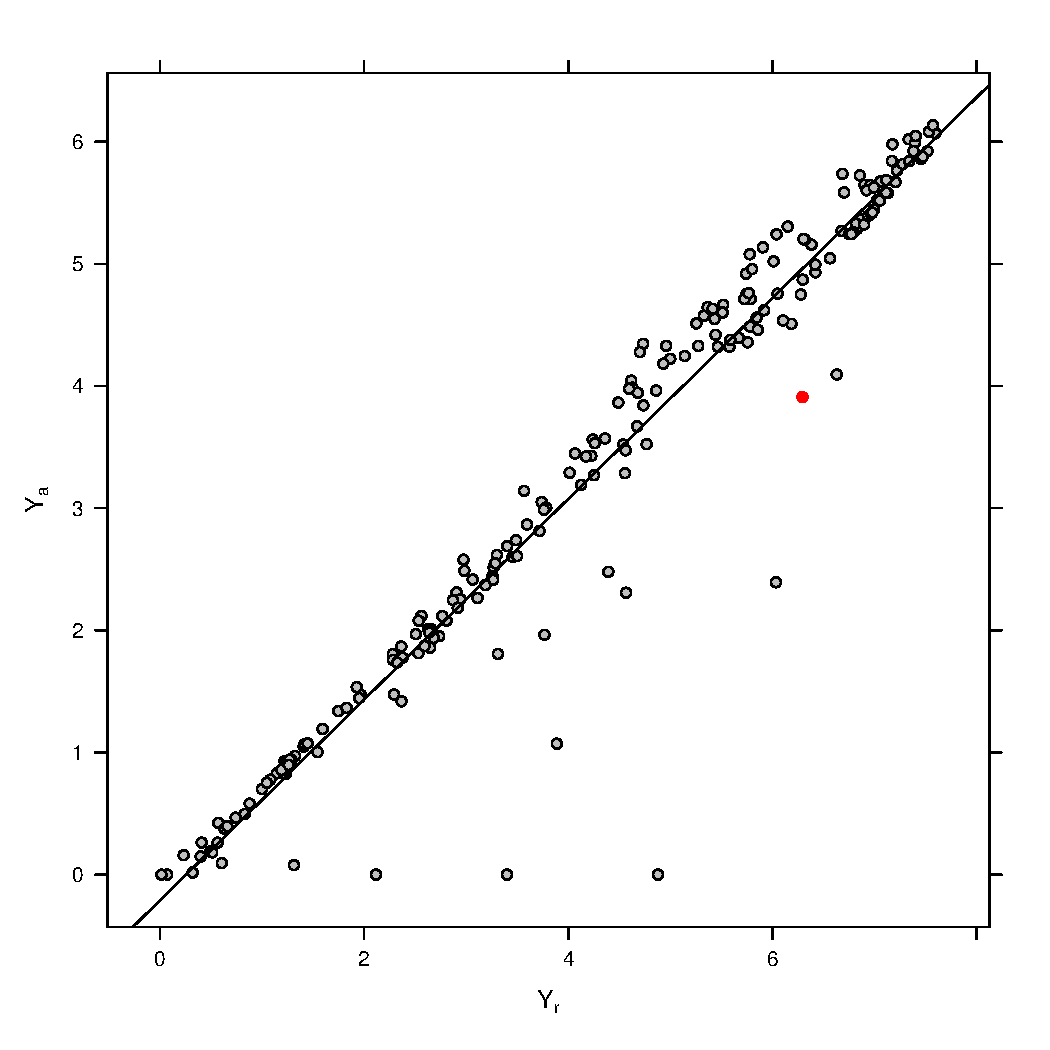
\includegraphics[height=0.95\textheight]{../figs/YaYr.pdf}
\end{center}
\end{column}
\end{columns}
\end{frame}

\begin{frame}[label={sec:orgc9123ac}]{Error de funcionamiento \(Y_a \sim Y_r\)}
\begin{center}
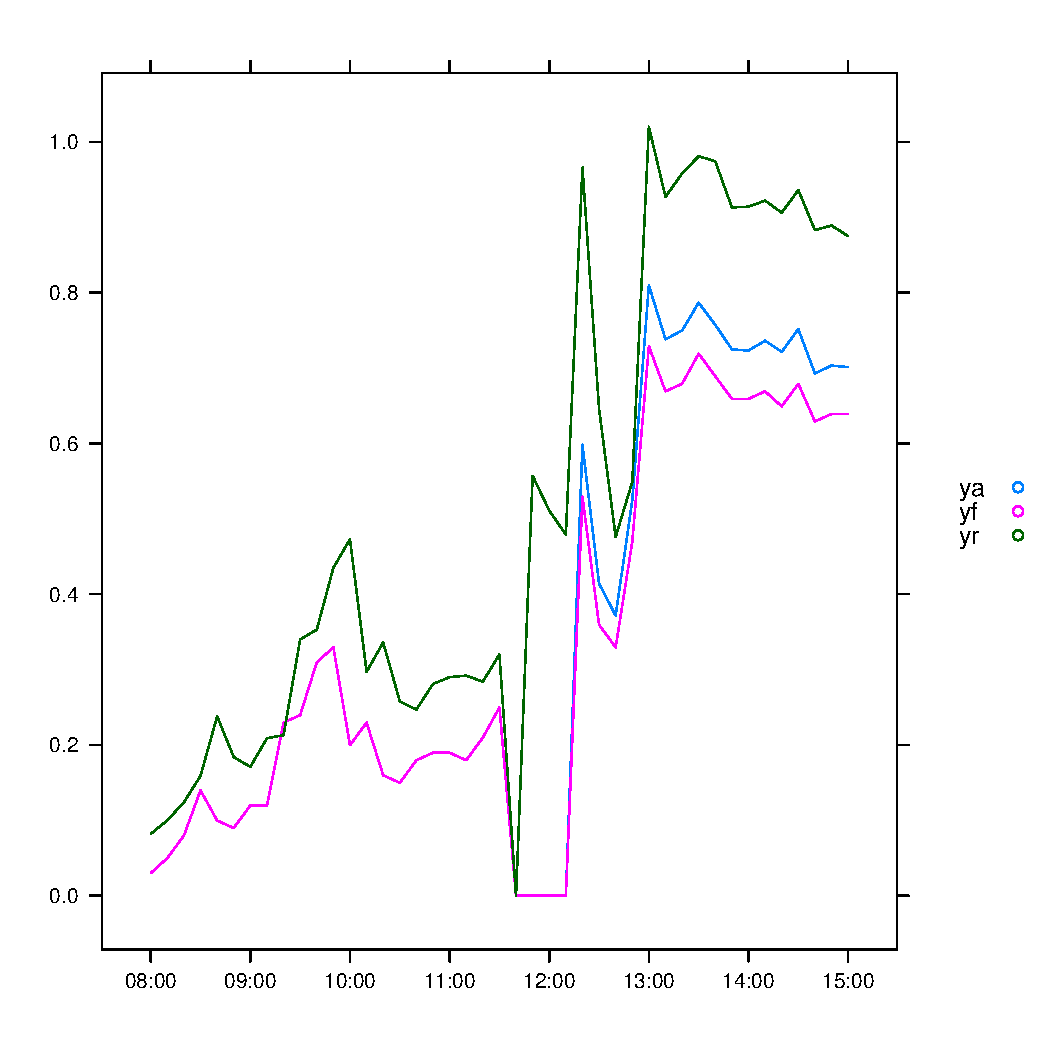
\includegraphics[height=0.95\textheight]{../figs/ErrorMonitorizacion.pdf}
\end{center}
\end{frame}


\begin{frame}[label={sec:orgbde23dd}]{\(pr \sim T_c\)}
\begin{columns}
\begin{column}{0.3\columnwidth}
\begin{itemize}
\item Valores intradiarios.
\item Relación lineal decreciente.
\item Detección de sombreado, degradación, o puntos calientes.
\end{itemize}
\end{column}

\begin{column}{0.7\columnwidth}
\begin{center}
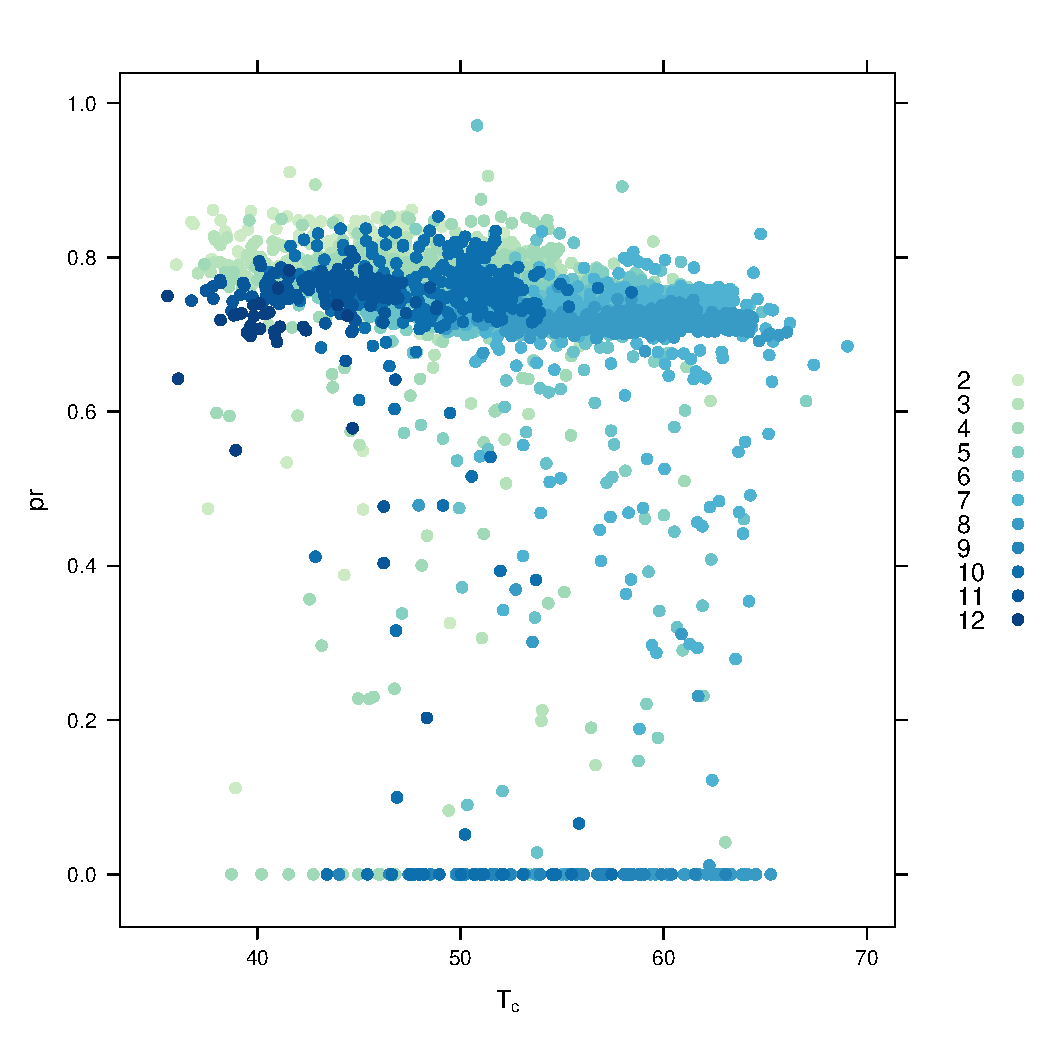
\includegraphics[height=0.95\textheight]{../figs/prTc.pdf}
\end{center}
\end{column}
\end{columns}
\end{frame}

\begin{frame}[label={sec:org2df4ebc}]{\(V_g \sim T_c\)}
\begin{columns}
\begin{column}{0.3\columnwidth}
\begin{itemize}
\item Valores intradiarios.
\item Relación lineal decreciente.
\item Detección de problemas en el MPPT, limitación del inversor, diodos de bypass.
\end{itemize}
\end{column}

\begin{column}{0.7\columnwidth}
\begin{center}
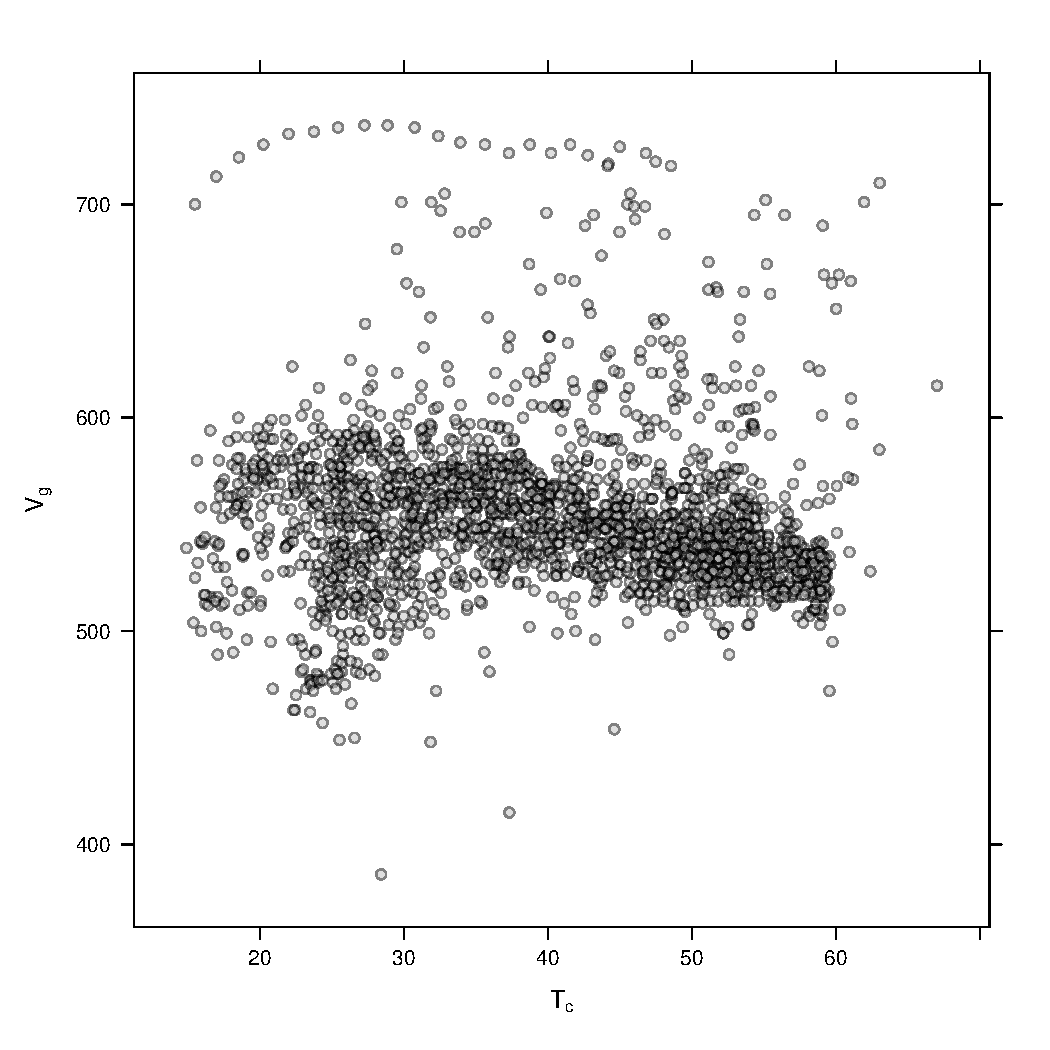
\includegraphics[height=0.95\textheight]{../figs/VgTc.pdf}
\end{center}
\end{column}
\end{columns}
\end{frame}

\begin{frame}[label={sec:org554f8b3}]{Error de funcionamiento \(V_g \sim T_c\)}
\begin{center}
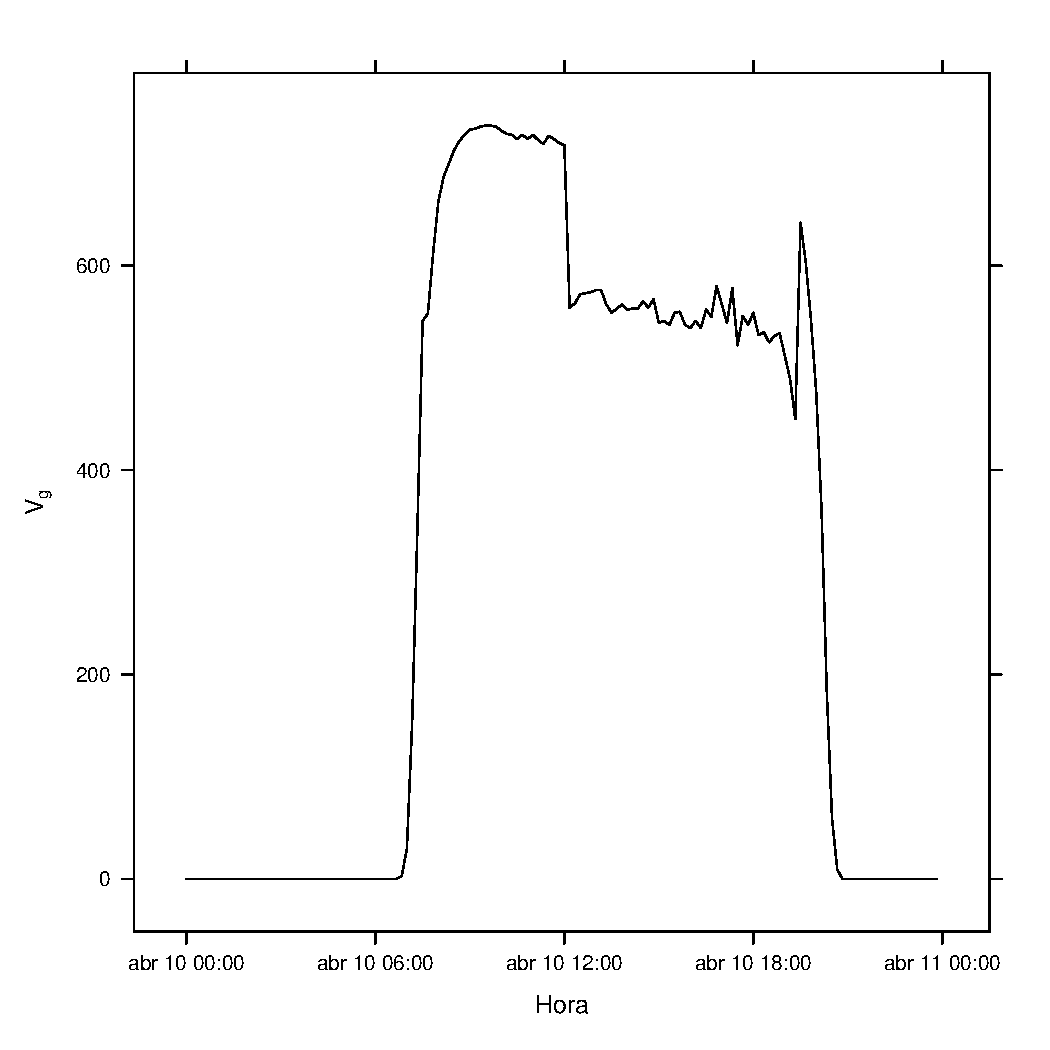
\includegraphics[height=0.95\textheight]{../figs/ErrorVgTc.pdf}
\end{center}
\end{frame}

\section{Comparación entre Datos y Estimación}
\label{sec:org9351dbd}

\begin{frame}[label={sec:orgb0667d0}]{Desviación entre modelo y observación}
\begin{itemize}
\item Sea \(O\) el conjunto de observaciones (medidas) de una variable aleatoria.
\end{itemize}

\[
\mathbf{O} = \left\{ o_1 \dots o_n \right\}
\]
\begin{itemize}
\item Sea \(M\) el conjunto de resultados de un modelo que aproxima el comportamiento de la variable medida.
\end{itemize}

\[
\mathbf{M} = \left\{ m_1 \dots m_n  \right\}
\]

\begin{itemize}
\item La desviación entre modelo y observación es:
\end{itemize}

\[
\mathbf{D} = \mathbf{M} - \mathbf{O} =  \left\{ (m_1 - o_1) \dots (m_n - o_n)  \right\} = \left\{ d_1 \dots d_n  \right\}
\]
\end{frame}

\begin{frame}[label={sec:org59f2a3d}]{Exactitud (\emph{bias}) y Precisión (\emph{variance})}
\begin{center}
\includegraphics[height=0.8\textheight]{../figs/bias-variance.png}
\end{center}

\url{http://scott.fortmann-roe.com/docs/BiasVariance.html}
\end{frame}

\begin{frame}[label={sec:org1a5a35b}]{Estimadores frecuentes: MBD y RMSD}
\begin{itemize}
\item Mean Bias Difference (MBD), diferencia media (indica si el modelo sobreestima o subestima):
\end{itemize}
\[
MBE = \overline{\mathbf{D}} = \overline{\mathbf{M}} - \overline{\mathbf{O}} = \frac{1}{n} \sum_{i=1}^n (m_i - o_i)
\]

\begin{itemize}
\item Root Mean Square Difference (RMSD), diferencia cuadrático media:
\end{itemize}
\[
RMSD = \left(\frac{1}{n} \sum_{i=1}^n d_i^2 \right)^{1/2} =  \left( \frac{1}{n} \sum_{i=1}^n (m_i - o_i)^2  \right)^{1/2}
\]
\end{frame}

\begin{frame}[label={sec:org0fc8b5a}]{Estimadores frecuentes: MBE y RMSD}
El RMSD agrega información del promedio y la varianza de la
  diferencia:
\[
RMSD^2= \overline{\mathbf{D}}^2 + \sigma^2_{\mathbf{D}} 
\]

donde la varianza de la diferencia (unbiased RMSD) se calcula:
\[
\sigma^2_{\mathbf{D}} = \frac{1}{n} \sum_{i=1}^n (d_i - \overline{\mathbf{D}})^2
\]
\end{frame}


\begin{frame}[label={sec:org58e28be}]{Otros estimadores: MAD}
\begin{itemize}
\item Mean Absolute Deviation (MAD):
\end{itemize}

\[
MAD = \frac{1}{n} \sum_{i=1}^n \left|d_i\right| =  \frac{1}{n} \sum_{i=1}^n \left|m_i - o_i\right|
\]
\begin{itemize}
\item El RMSD no es robusto (un error puntual puede distorsionar el estimador) y depende del número de muestras\footnote{\url{https://www.int-res.com/abstracts/cr/v30/n1/p79-82/}

\url{https://doi.org/10.1016/j.atmosenv.2008.10.005}}:
\end{itemize}
\[
MAD \leq RMSD \leq n^{1/2} MAD
\]
\end{frame}

\begin{frame}[label={sec:org08c60d9}]{Correlación}
El coeficiente de correlación entre dos conjuntos de datos es una
medida numérica de la relación \alert{lineal} entre los dos conjuntos (si la
relación no es lineal, este coeficiente no sirve):

\begin{columns}
\begin{column}{0.5\columnwidth}
\[
r = \frac{1}{n-1} \cdot \sum_{i=1}^{n} \left( \frac{o_{i}-\overline{\mathbf{O}}}{\sigma_{\mathbf{O}}}\right) \cdot \left(\frac{m_{i}-\overline{\mathbf{M}}}{\sigma_{\mathbf{M}}}\right)
\]
\end{column}

\begin{column}{0.5\columnwidth}
\begin{center}
\includegraphics[height=0.7\textheight]{../figs/Splom.png}
\end{center}
\end{column}
\end{columns}
\end{frame}


\section{Coherencia Estadística}
\label{sec:org4378f75}

\begin{frame}[label={sec:orgebcf1b6}]{Planteamiento}
\begin{itemize}
\item En un sistema compuesto por diferentes \alert{unidades idénticas}, el funcionamiento de todas ellas debe ser el mismo.
\item Los \alert{elementos reales} presentan \alert{diferencias} (tolerancia de potencia, pérdidas de dispersión, suciedad), de forma que el comportamiento de cada unidad se desviará del comportamiento promedio.
\item Si \alert{no hay problemas de funcionamiento}, estas desviaciones no superarán un umbral determinado (\alert{coherencia estadística}).
\item Un análisis estadístico del funcionamiento del conjunto puede \alert{identificar una unidad defectuosa} como aquella que se aparta significativamente del comportamiento promedio.
\end{itemize}
\end{frame}
\begin{frame}[label={sec:org7e768f5}]{Coherencia estadística}
\begin{itemize}
\item Una medida puede ser etiquetada como \emph{outlier} si es poco probable que pertenezca a la misma distribución que el conjunto.
\item En estadística hay métodos diversos para realizar este análisis:
\begin{itemize}
\item Métodos gráficos
\item Teorema de Chebyshev.
\item Criterios de Pierce y Chauvenet
\end{itemize}
\item Los criterios de Pierce y Chauvenet asumen \alert{distribución gaussiana} (aceptable en nuestro contexto) y son \alert{simples de implementar}, particularmente Chauvenet.
\end{itemize}
\end{frame}


\begin{frame}[label={sec:orgb6e2511}]{Método de Chauvenet}
Una medida es un \emph{outlier} si la probabilidad de obtener su desviación
respecto de la media es inferior al inverso de 2 veces el número de
elementos en el conjunto.
\begin{center}
\includegraphics[height=0.6\textheight]{../figs/chauvenet.png}
\end{center}
\end{frame}

\begin{frame}[label={sec:org731c1e5}]{Método de Chauvenet\footnote{\url{https://doi.org/10.1016/j.solener.2009.08.008}}}
\begin{enumerate}
\item Supongamos un SFV compuesto por \(N\) unidades idénticas.
\item Sea \(Y_{f,i}\) la medida de \alert{productividad diaria} de una de esas unidades.
\item Se calcula la \alert{media}, \(\overline{Y}_f\), y la \alert{desviación estándar}, \(\sigma_{Y_f}\), del \alert{conjunto}.
\item Se calcula la \alert{distancia estadística} de cada unidad respecto del sistema total:
\[
d_i = \frac{Y_{f,i} - \overline{Y}_f}{\sigma_{Y_f}}
\]
\item En una distribución gaussiana, se calcula la distancia estadística
equivalente a la probabilidad límite de Chauvenet, \(1/2N\), teniendo en cuenta
que hay dos colas.
\item Aquellas observaciones que superan la distancia son \alert{marcadas como outliers}.
\end{enumerate}
\end{frame}


\begin{frame}[label={sec:org0614079}]{Método de Chauvenet}
\begin{itemize}
\item Por ejemplo, para un sistema de 10 unidades, la probabilidad es \(1/20\).

\item A cada cola le corresponde la mitad, \(1/40 = 0.025\).

\item Por tanto, el límite es \(d_{max} = - 1.9599\) (cola izquierda, valores por debajo del conjunto).
\end{itemize}


\begin{columns}
\begin{column}{0.3\columnwidth}
\[
  d_i = \frac{Y_{f,i} - \overline{Y}_f}{\sigma_{Y_f}}
\]

\[
\left| d_i \right| > \left| d_{max} \right|
\]
\end{column}

\begin{column}{0.8\columnwidth}
\begin{center}
\begin{center}
\includegraphics[width=.9\linewidth]{../figs/chauvenet.png}
\end{center}
\end{center}
\end{column}
\end{columns}
\end{frame}

\begin{frame}[label={sec:org9e0d24e}]{Métodos gráficos: Target Diagram\footnote{\url{https://doi.org/10.1016/j.jmarsys.2008.05.014}}}
\begin{itemize}
\item Emplea la relación entre \(RMSD\), \(\sigma^2_{\mathbf{D}}\), y \(\overline{\mathbf{D}}\), normalizadas con \(\sigma_{\mathbf{O}}\):
\end{itemize}
  \[
  RMSD' = RMSD / \sigma_{\mathbf{O}}
  \]
\[
  \sigma'_{\mathbf{D}} = \sigma_{\mathbf{D}} / \sigma_{\mathbf{O}} 
\]
\[
\overline{\mathbf{D}}' = \overline{\mathbf{D}} / \sigma_{\mathbf{O}}
\]
\[
RMSD'^2= \sigma'^2_{\mathbf{D}} + \overline{\mathbf{D}}'^2
\]

\begin{itemize}
\item Incorpora el signo de la diferencia entre desviaciones estándar del modelo y las observaciones.
\end{itemize}
\[
sign_{\sigma} =  sign(\sigma_{\mathbf{M}} - \sigma_{\mathbf{O}} )
\]
\end{frame}


\begin{frame}[label={sec:orgbf49654}]{Métodos gráficos: Target Diagram}
\begin{columns}
\begin{column}{0.4\columnwidth}
\begin{itemize}
\item \(\sigma'_{\mathbf{D}}\) (con signo): Eje horizontal
\item \(\overline{\mathbf{D}}'\): Eje vertical
\item \(RMSD'^2\): Distancia al origen
\end{itemize}
\end{column}

\begin{column}{0.6\columnwidth}
\begin{center}
\includegraphics[height=0.9\textheight]{../figs/TargetDiagram.pdf}
\end{center}
\end{column}
\end{columns}
\end{frame}


\begin{frame}[label={sec:org9eec429}]{Ejemplo de uso de Target Diagram}
\begin{itemize}
\item Sea \(Y_{f,i}(t)\) la serie temporal de la productividad diaria de \alert{una unidad} del SFV.
\item Sea \(\widetilde{Y}_{f}(t)\) la serie temporal de la \alert{mediana} de la productividad diaria del SFV \alert{completo}.
\item Tomando \(\widetilde{Y}_{f}(t)\) como modelo o referencia, podemos
emplear diagramas para detectar unidades defectuosas durante diferentes
períodos de tiempo.
\end{itemize}

\begin{center}
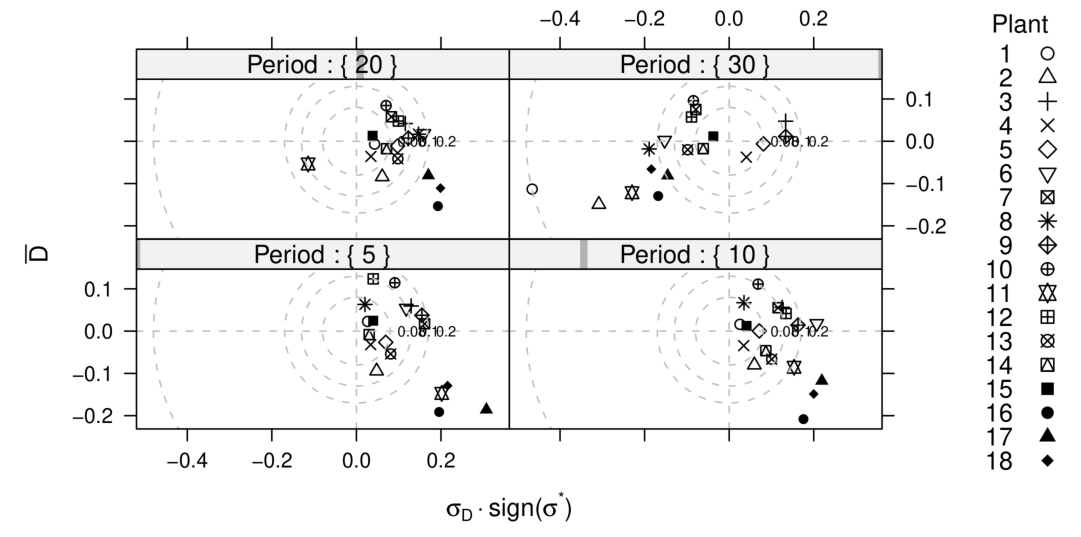
\includegraphics[height=0.6\textheight]{../figs/TargetDiagram_Dia120.pdf}
\end{center}
\end{frame}
\end{document}
